
\subsection{Ordonnancement et heuristique}

Il est important de remarquer que les séances peuvent être ordonnées avant de
chercher une planification. Les séances d'une même matière se suivant, il est
intéressant de commencer par planifier la première, puis la seconde, etc.

Le prédicat \texttt{indiceSeance(+S, -I)} implémente donc l'heuristique
retournant l'indice d'une séance dans l'arbre des séances séquencées. Cette
heuristique nous permet de trier les séances à priori et de commencer la
la planification des séances de plus petits indices. Elles doivent logiquement
se dérouler en début de période scolaire.

Cet ordonnancement nous permet de rapidement partir dans une branche
relativement bonne. Sans ordonnancement, on peut voir le moteur d'inférence
commencer par placer la dernière séance d'une matière sur le premier
créneau de l'année, ce qui entraine alors de très nombreux retours arrières.

Cela revient un peu à trier les séances selon un critère de contrainte (leur
dépendance aux séances précédentes). L'originalité est ici qu'on ne commence pas
par les plus contraintes, mais par les plus libres, à cause de l'aspect temporel
du problème.

\begin{figure}[H]
    \centering
    \subfloat[Sans ordonnancement]{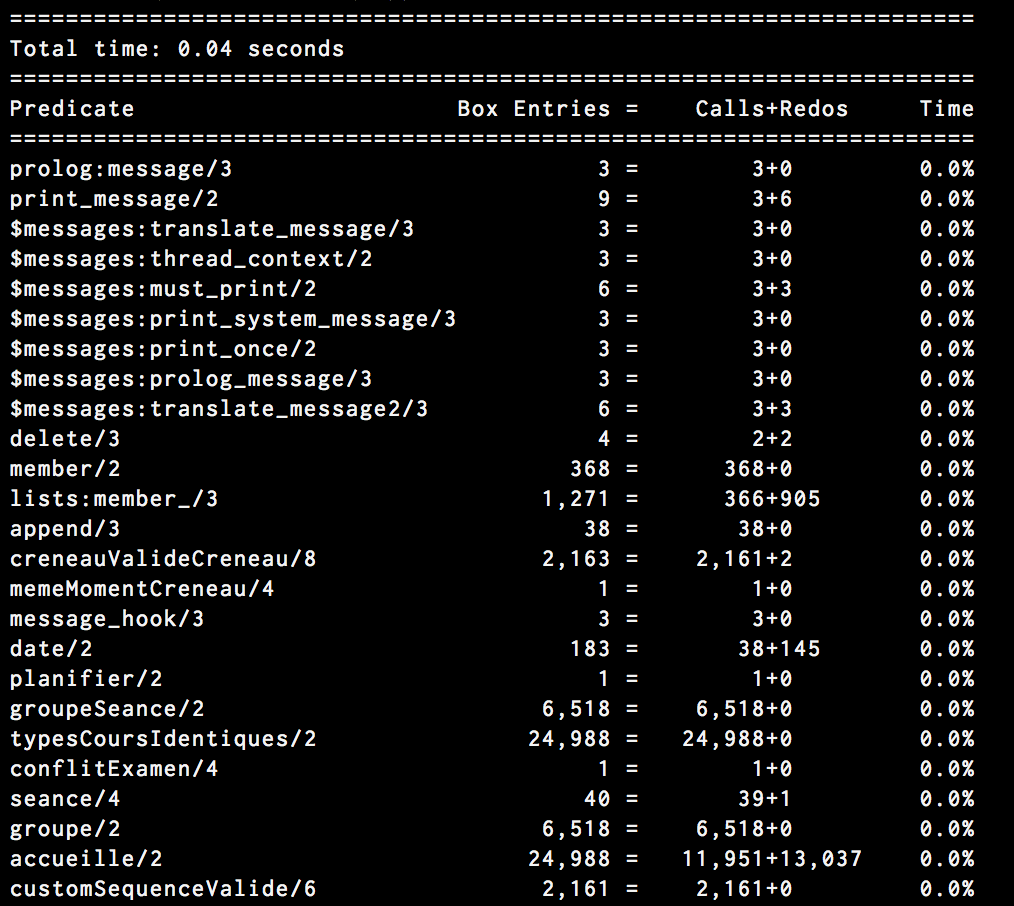
\includegraphics[width=7cm]{noordering.png}}
    \subfloat[Avec ordonnancement]{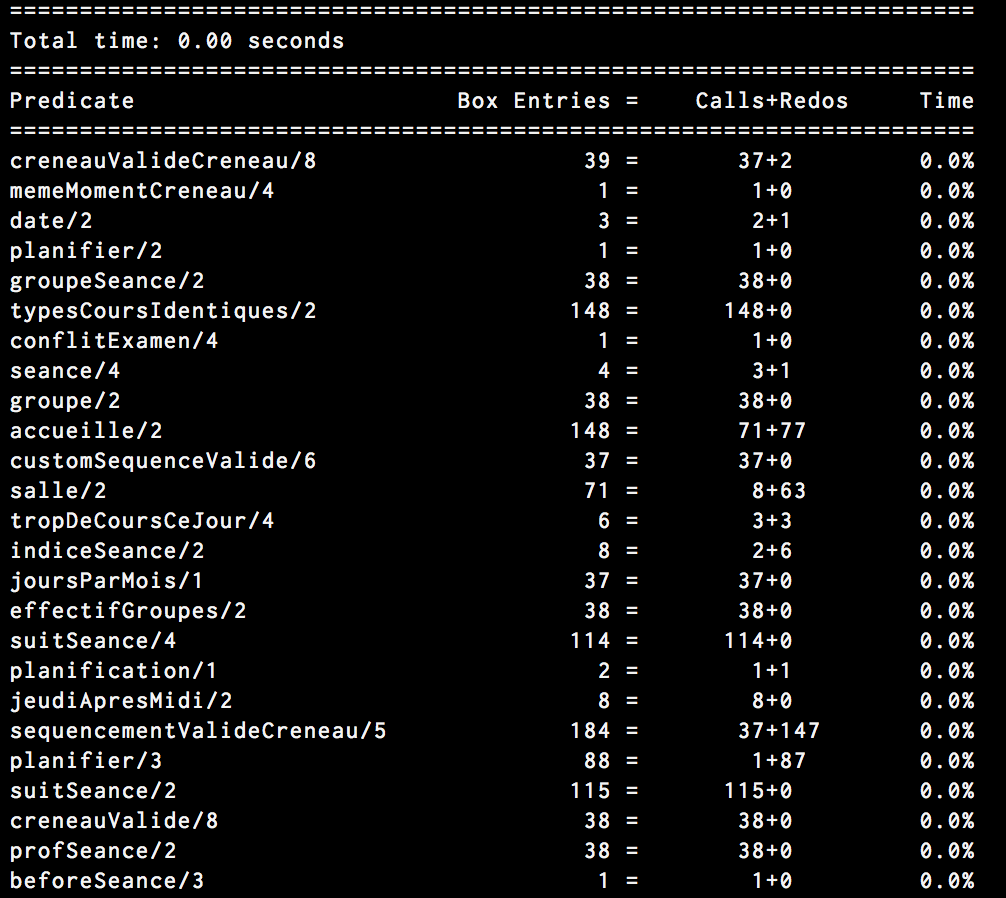
\includegraphics[width=7cm]{ordering.png}}
    \caption{\label{fig:orderingcompare} Comparaison sans/avec ordonnancement}
\end{figure}

Sur la figure \ref{fig:orderingcompare}, on compare deux profiling d'un jeu de
données très simple (2 séances S1 et S2, S2 suit S1), à gauche, sans
ordonnancement, à droite, avec.  On remarque par exemple un nombre bien plus
important de "Calls+Redos" sur \texttt{creneauValideCreneau} ou
\texttt{typesCoursIdentiques} à gauche.

En effet, l'algorithme a eu le malheur
d'assigner la séance S2 au premier moment disponible et à tester toutes les
créneaux possibles pour S1 avant d'effectuer un retour arrière et mettre S1 en
premier.
C'est le genre de situation que l'ordonnancement permet d'éviter.
